\documentclass{article}
\usepackage{graphicx}

\title{Data Analysis Project Report - Week 2}
\author{Shrestha, Prashant; Vahteristo, Ilmari; Vanegas, Sergio}

\begin{document}

\maketitle

\section{Introduction} % Talk about communication channel and data import

\section{Dataset analysis}

\section{Data visualisation}

\section{Data treatment}
The preprocessing of the mining dataset for predicting the outlet silica concentration involves addressing two primary challenges:
fixing abnormal functioning time series data and dealing with the dissimilar frequencies within the time series.

\subsection{Fixing Abnormalities in Time Series Data}

There is an absence of samples between March 16 at 05:00 and March 29 at 12:00.
The abnormalities in this section of the dataset can be fixed using two options:
Imputation or removal. Since the abnormalities are situated at the beginning of the time series and constitute only
3.63 percentage of the total dataset, the section of the dataset is removed for further analysis. 
Furthermore, following the removal of the section, we encounter a missing sample for the time April 10, at 00:00. 
To fix the missing sample, we imputed the data with the last sample hour. Figure~\ref{fig:Missing_sample_1} 
and Figure~\ref{fig:Missing_sample_2} depicts the absence of the sample in the dataset. Figure~\ref{fig: Intrapolation} 
shows the imputation of data for the missing sample for April 10, at 00:00.

begin{figure}[h] 
  \centering
  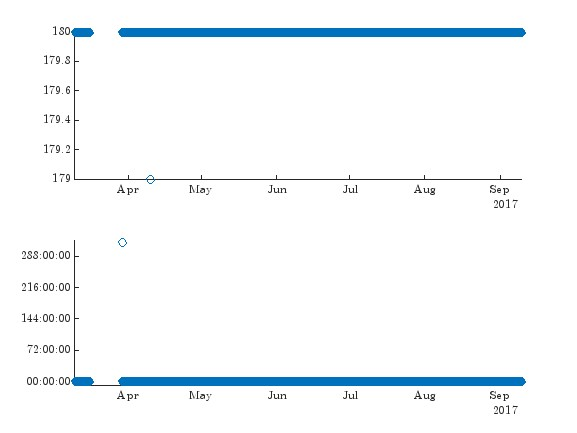
\includegraphics[width=0.6\textwidth]{Missing_sample_1.jpg}
  \caption{Missing_sample_1}
  \label{fig:Missing_sample_1}
\end{figure}

begin{figure}[h] 
  \centering
  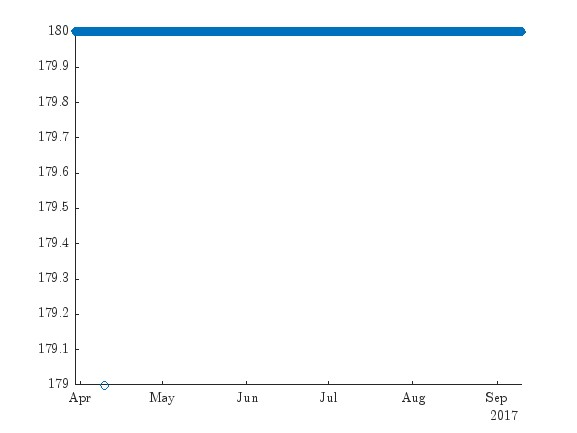
\includegraphics[width=0.6\textwidth]{Missing_sample_2.jpg}
  \caption{Missing_sample_2}
  \label{fig:Missing_sample_2}
\end{figure}
\subsection{Dealing with Dissimilar Frequencies in the Time Series}

begin{figure}[h] 
  \centering
  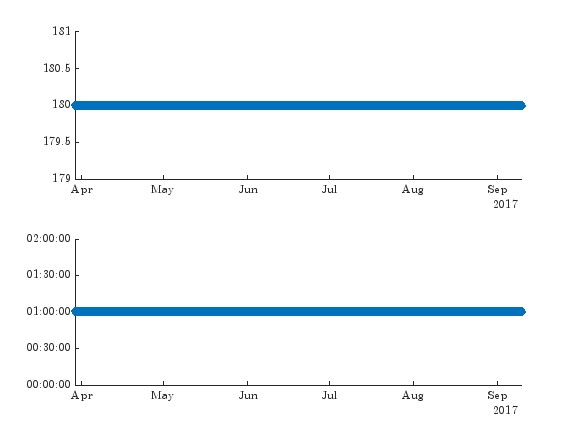
\includegraphics[width=0.6\textwidth]{Intrapolation_1.jpg}
  \caption{Intrapolation}
  \label{fig: Intrapolation}
\end{figure}
\subsection{Dealing with Dissimilar Frequencies in the Time Series}

From the descriptions of the dataset, we know that the observation for some features changes every 20 seconds,
while some features remain constant for an hour. The problem can be effectively addressed through resampling, 
which includes both down-sampling and up-sampling methods. For up-sampling, we assume that the initial sample 
is collected at the 0th second of the hour, with subsequent samples captured regularly at 20-second intervals. 
We can rectify the up-sampling process by adjusting the timestamp in the dataset. However, for down-sampling, 
we are considering two different approaches. One of the methods involves the calculation of hourly medians for 
each sample, and the other method involves the aggregation of feature data into hourly vectors. 
The choice between the two approaches, up-sampling and down-sampling, will depend on the project's 
specific prediction goal: whether it is to forecast silica ore concentration every 20 seconds or every hour.

\end{document}